\section{Vulnerability: JavaScript Injection Attack}
\label{sec:background}
\textbf{Description:} A second type of injection attack works on this website. It was possible to enter a JavaScript script into the transaction box. This would be stored by
the database as the description of the transaction. Consequently when the user clicked \textit{List transactions} each transaction would be listed, and as such each description
interpreted in html. This means a description enclosed by \verb|<script></script>| tags will be interpreted as a script and as such executed as the website comes to list the
transactions. This allows a hacker to gain valuable information by printing out session data in a pop up window. This security flaw is exasperated by the fact that all transactions
are viewable to all users. Thus any script injected will affect all users. This is known as a persistent (or stored) vulnerability. Persistent vulnerabilities are more significant
since the malicious script is rendered automatically, therefore there is no requirement to individually target victims or to take them to a third party website.\\ \\
\textbf{Testing the Vulnerability:} To test this vulnerability a series of JavaScript queries were entered as transactions. One of the most dangerous was the following:
\begin{minted}{html}
   <script>alert(document.cookie)</script>
\end{minted}
Once injected upon the selection of \textit{List transactions} this will open a popup window which will display the users token.
\begin{figure}[h]
   \centering
   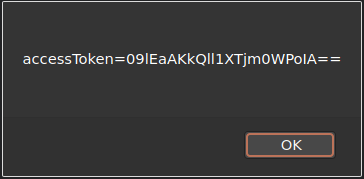
\includegraphics[width=0.5\textwidth]{figs/popup.png}
   \caption{The popup window displayed when a user clicks \textit{List transactions}}
   \label{popup}
\end{figure}\\
As can be seen from this figure, this injecton allows a user to display the token. This again being particularly dangerous since the tokens are not time dependent on this website.
Consequently this can be said to be a major security flaw since it has the possibility of allowing a hacker indefinite access to the banking website.\\ \\
\textbf{Mitigation:} 
 
